\documentclass[resume]{subfiles}


\begin{document}
\section{Différences finies}
\subsection{Différences finies progressives (downwind)}
\subsubsection{$f'(x)$}
\begin{figure}[H]
\centering
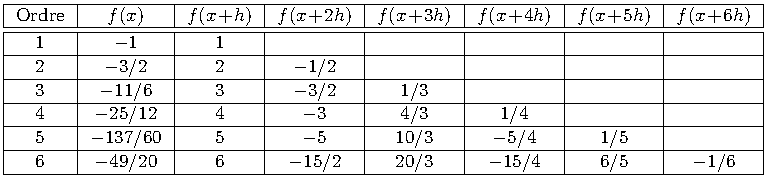
\includegraphics[width=\columnwidth,page=1]{diff_finies_tableaux.pdf}
\end{figure}
$\textcolor{ForestGreen}{n=2}$
$$f\textcolor{OrangeRed}{'}(x)=\frac{-\frac{3}{2}f(x)+2f(x+h)-\frac{1}{2}f(x+2h)}{\textcolor{OrangeRed}{h}}+\mathcal{O}(h^{\textcolor{ForestGreen}{2}})$$
\subsubsection{$f''(x)$}
\begin{figure}[H]
\centering
\includegraphics[width=\columnwidth,page=2]{diff_finies_tableaux.pdf}
\end{figure}
$\textcolor{ForestGreen}{n=3}$
$$f\textcolor{OrangeRed}{''}\left(x\right)=\frac{\splitdfrac{\splitdfrac{\frac{35}{12}f\left(x\right)}{-\frac{26}{3}f\left(x+h\right)+\frac{19}{2}f\left(x+2h\right)}}{-\frac{14}{3}f\left(x+3h\right)+\frac{11}{12}f\left(x+4h\right)}}{h^{\textcolor{OrangeRed}{2}}}+\mathcal{O}(h^{\textcolor{ForestGreen}{3}})$$
\subsubsection{$f'''(x)$}
\begin{figure}[H]
\centering
\includegraphics[width=\columnwidth,page=3]{diff_finies_tableaux.pdf}
\end{figure}
$\textcolor{ForestGreen}{n=1}$
$$f\textcolor{OrangeRed}{'''}\left(x\right)=\frac{\splitdfrac{-f\left(x\right)+3f\left(x+h\right)}{-3f\left(x+2h\right)+f\left(x+3h\right)}}{h^{\textcolor{OrangeRed}{3}}}+\mathcal{O}(h^{\textcolor{ForestGreen}{1}})$$
\subsection{Différences finies rétrogrades (upwind)}
\begin{enumerate}
\item Remplacer $x+kh$ par $x-kh$
\item Si dérivée paire : Pas de changement de coefficient
\item Si dérivée impaire : Changement du signe
\end{enumerate}
\subsection{Différences finies centrées}
\subsubsection{$f'(x)$}
\begin{figure}[H]
\centering
\includegraphics[width=\columnwidth,page=5]{diff_finies_tableaux.pdf}
\end{figure}
$\textcolor{ForestGreen}{n=2}$
$$f\textcolor{OrangeRed}{'}(x)=\frac{-\frac{1}{2}f(x-h)+\frac{1}{2}f(x+h)}{h^{\textcolor{OrangeRed}{1}}}+\mathcal{O}(h^{\textcolor{ForestGreen}{2}})$$
\subsubsection{$f''(x)$}
\begin{figure}[H]
\centering
\includegraphics[width=\columnwidth,page=6]{diff_finies_tableaux.pdf}
\end{figure}
$\textcolor{ForestGreen}{n=2}$
$$f\textcolor{OrangeRed}{''}(x)=\frac{f(x-h)-2f(x)+f(x+h)}{h^{\textcolor{OrangeRed}{2}}}+\mathcal{O}(h^{\textcolor{ForestGreen}{2}})$$
\subsubsection{$f'''(x)$}
\begin{figure}[H]
\centering
\includegraphics[width=\columnwidth,page=7]{diff_finies_tableaux.pdf}
\end{figure}
$\textcolor{ForestGreen}{n=2}$
$$f\textcolor{OrangeRed}{'''}(x)=\frac{\splitdfrac{-\frac{1}{2}f(x-2h)+f(x-h)}{-f(x+h)+\frac{1}{2}f(x+2h)}}{h^{\textcolor{OrangeRed}{3}}}+\mathcal{O}(h^{\textcolor{ForestGreen}{2}})$$
\subsection{Différences finies pour EDP elliptiques + Dirichlet}
$$-u''(x)=f(x)\qquad u(0)=\alpha\quad u(L)=\beta$$,
$$u''(x_j)\approx\frac{u(x_j-h)-2u(x_j)+u(x_j+h)}{h^2}$$
Ce qui donne un système d'équations linéaires
$$\frac{1}{h^2}\begin{pmatrix}
2 & -1 & 0 & \cdots & 0\\
-1 & 2 & -1 & \cdots & 0\\
\vdots & \vdots & \ddots & \vdots & \vdots\\
0 & 0 & 0 & \ddots & -1\\
0 & 0 & 0 & \cdots & 2
\end{pmatrix}\begin{pmatrix}u_1\\u_2\\\vdots\\u_n\end{pmatrix}=\begin{pmatrix}f(x_1)+\frac{\alpha}{h^2}\\f(x_2)\\\vdots\\f(x_n)+\frac{\beta}{h^2}\end{pmatrix}$$
$$A_h\vec{x}=\vec{f}$$
\textcolor{OrangeRed}{les valeurs sont inversées car $-u''(x)$}.
\subsubsection{2D}
$$u_{xx}(x_i,y_j)\approx\frac{u(x_i-h,y_j)-2u(x_i,y_j)+u(x_i+h,y_j)}{h^2}$$
$$u_{yy}(x_i,y_j)\approx\frac{y(x_i,y_j-h)-2u(x_i,y_j)+u(x_i,y_j+h)}{h^2}$$
\subsection{Différences finies pour EDP paraboliques}
\begin{enumerate}
\item Discrétiser l'espace (sous-intervalles de largeur $h$)
\item Application des conditions aux bords puis recherche des valeurs aux nœuds en fonction du temps
$$x_i\to u_i(t)$$
$$u_i(t)\approx u(x_i,t)$$
\item On applique les conditions initiales
$$u_i(0)=u_0(x_i)$$
\item Résoudre le problème de Cauchy ($\frac{du}{dt}=g(x,t)$ en matrices)
\end{enumerate}
\subsection{Méthode d'Euler explicite}
$$\frac{du}{dt}=F(t_0,u_0)$$
Vu d'un autre angle, on veut approcher
$$\frac{d}{dt}\vec{u}(t)\approx \frac{u(t_i+\tau)-u(t_i)}{\tau}$$
\subsection{Relation entre le pas de temps et le pas temporel}
$$\tau\leq \frac{h^2}{2\mu}$$
Avec $\mu$ la constante de l'équation $u_t-\mu u_{xx}=f(x,t)$
\subsection{Équation de transport}
$$v\leq \frac{h}{\tau}\longleftrightarrow \frac{v\tau}{h}=r\leq 1$$
C'est la condition CFL : avec downwind c'est impossible de résoudre le problème. Avec les upwind on peut y arriver parce qu'on utilise les valeurs précédentes (la condition sur $v$ reste valable).\\
L'analyse de Von Neumann montre que le schéma centré n'est pas stable (même si la condition CFL est vérifiée).

\subsection{Exemple Différences finies}
\begin{align*} % exercice3 serie8 exemple de différence finies
-u''(x) = f(x) = (3x+x^2)e^x \textbf{Avec CB (D) = 0}\\
h=1/5 \rightarrow 0 \frac{1}{5} \frac{2}{5} \frac{3}{5} \frac{4}{5} 1
\end{align*}
\subsection{méthode d'Euler}
$$\vec{u}_{k+1}=\vec{u}_k+\tau\left(-A\vec{u}_k+\vec{b}(t_k)\right)$$
\subsection{Méthode d'Euler implicite}
$$\vec{u}_{k+1}=\vec{u}_k+\tau\left(-A\vec{u}_{k+1}+\vec{b}(t_{k+1})\right)$$
Vérifier les formules... c'est illisible sur le polycop
\end{document}